\chapter{Trous noirs, trous blancs et diagramme causal global}

\lectureoverview{Un horizon est ordinaire localement, mais décisif à l’échelle globale. Nous partons de la métrique de Schwarzschild près de l’horizon, la suivons vers l’extérieur à l’aide de l’analogie du cigare euclidien, puis nous demandons ce qu’Alice et Bob peuvent réellement observer. La singularité et la région du trou blanc, renversée dans le temps, étendent cette image locale à l’espace-temps de Schwarzschild éternel. La compactification de Penrose rend la structure causale finie et lisible. Enfin, nous passons d’une solution éternelle à un trou noir formé par effondrement, où le théorème des coquilles de Newton et le théorème de Birkhoff fournissent les éléments à raccorder.}

\section{De l’horizon à l’infini}

Au voisinage d’un horizon de Schwarzschild suffisamment grand, la courbure est faible à l’échelle d’un petit laboratoire et la géométrie radiale-temporelle est approximativement plate. La variable radiale la plus commode n’est pas la coordonnée de Schwarzschild \(r\), mais la distance propre \(\rho\) mesurée vers l’extérieur à partir de l’horizon, le long d’une tranche spatiale à temps constant :
\begin{equation}
\rho=0 \quad\Longleftrightarrow\quad r=2GM .
\label{eq:l04-rho-horizon}
\end{equation}
La coordonnée temporelle la plus commode est la quantité sans dimension
\begin{equation}
\omega=\frac{t}{4GM},
\label{eq:l04-omega}
\end{equation}
où \(c=1\). Ainsi, \(\omega\) est le temps de Schwarzschild exprimé en unités de deux fois le rayon de Schwarzschild.

Avec la convention où la signature est surtout positive, la métrique radiale-temporelle près de l’horizon s’écrit
\begin{equation}
ds^2\approx-\rho^2d\omega^2+d\rho^2.
\label{eq:l04-rindler}
\end{equation}
La 2-sphère angulaire a été omise, car le présent argument ne porte que sur le temps et la distance radiale.

\begin{figure}[htbp]
\centering
\includegraphics[width=0.72\textwidth]{lecture_04_figure_02.png}
\caption{La métrique près de l’horizon et le temps de Schwarzschild redimensionné.}
\lectureframe{00:05:46.800}
\end{figure}

L’équation~\eqref{eq:l04-rindler} est à l’espace-temps de Minkowski ce que les coordonnées polaires sont au plan euclidien. Pour
\begin{equation}
T=\rho\sinh\omega,
\qquad
X=\rho\cosh\omega,
\end{equation}
on obtient
\begin{equation}
-dT^2+dX^2=-\rho^2d\omega^2+d\rho^2.
\end{equation}
Les lignes où \(\rho\) est constant sont des hyperboles \(X^2-T^2=\rho^2\), tandis que \(\omega\) s’étend du passé lointain au futur lointain. Les deux droites nulles \(X=\pm T\) se rencontrent au point de bifurcation du diagramme réduit. En quatre dimensions, ce point représente une 2-sphère, et les deux nappes nulles future et passée forment un horizon de Killing bifurqué.\editorialnote{Dans le diagramme radial, il est commode, par abus de langage, d’appeler horizon bifurqué le seul point d’intersection. Plus précisément, les deux branches de l’horizon se coupent sur une 2-sphère de bifurcation.}

\subsection{La région lointaine}

La partie radiale-temporelle de la métrique de Schwarzschild est
\begin{equation}
ds^2
=-\left(1-\frac{2GM}{r}\right)dt^2
+\frac{dr^2}{1-\frac{2GM}{r}}.
\label{eq:l04-schwarzschild}
\end{equation}
Loin du trou, \(r\gg2GM\), la métrique tend vers
\begin{equation}
ds^2\approx-dt^2+dr^2.
\end{equation}
Là, \(r\) et \(\rho\) ne diffèrent que par une correction additive sans importance ; ainsi, avec \(dt=4GM\,d\omega\),
\begin{equation}
ds^2\approx-(4GM)^2d\omega^2+d\rho^2.
\label{eq:l04-far}
\end{equation}
Le coefficient radial est simple dans les deux limites. C’est le coefficient temporel qui change :
\begin{equation}
ds^2\approx
\begin{cases}
-\rho^2d\omega^2+d\rho^2, & \rho\ll GM,\\[3pt]
-(4GM)^2d\omega^2+d\rho^2, & \rho\gg GM.
\end{cases}
\label{eq:l04-two-limits}
\end{equation}
Le long d’une trajectoire en stationnaire, \(d\rho=0\). Près de l’horizon,
\begin{equation}
d\tau=\rho\,d\omega,
\end{equation}
tandis que loin de celui-ci \(d\tau\approx4GM\,d\omega=dt\). Pour un intervalle fixé de la coordonnée temporelle extérieure, le temps propre écoulé sur une horloge maintenue près de l’horizon devient de plus en plus court.

\subsection{Le cigare}

L’espace-temps est difficile à se représenter ; remplaçons donc la direction temporelle par une direction angulaire ordinaire. Écrivons
\begin{equation}
\begin{aligned}
d\ell^2&=F(\rho)^2d\theta^2+d\rho^2,\\
F(\rho)&\sim
\begin{cases}
\rho, & \rho\to0,\\
4GM, & \rho\to\infty.
\end{cases}
\end{aligned}
\label{eq:l04-cigar}
\end{equation}
Au voisinage de \(\rho=0\), il s’agit du plan en coordonnées polaires. Loin de là, la circonférence ne croît plus avec le rayon :
\begin{equation}
C_\infty=\int_0^{2\pi}4GM\,d\theta=8\pi GM.
\label{eq:l04-cigar-circumference}
\end{equation}
La surface s’arrondit donc à une extrémité et tend vers un cylindre à l’autre. Elle ressemble à un cigare.

\begin{figure}[htbp]
\centering
\includegraphics[width=0.74\textwidth]{lecture_04_figure_03.png}
\caption{Comparaison euclidienne : une extrémité polaire reliée à un cylindre asymptotique de circonférence \(8\pi GM\).}
\lectureframe{00:14:05.000}
\end{figure}

Plus la masse est grande, plus la circonférence asymptotique est grande et plus la courbure près de l’extrémité est douce. Un petit trou correspond à un cigare fortement courbé ; un grand trou a une extrémité large et faiblement courbée. Il s’agit d’une représentation de l’interpolation de l’équation~\eqref{eq:l04-two-limits}, et non d’un plongement du trou noir lorentzien lui-même.\editorialnote{L’objet géométrique précis s’obtient en prolongeant le temps de Schwarzschild en temps imaginaire. La régularité à l’extrémité fixe alors la période du temps euclidien à \(8\pi GM\), soit la même échelle que celle qui détermine ensuite la température de Hawking. Dans ce cours, l’analogie n’est utilisée ici qu’à titre visuel.}

\section{Lire l’horizon du point de vue causal}

À l’extérieur du trou, \(\rho>0\), un observateur stationnaire suit une hyperbole à \(\rho\) constant. Loin de l’horizon, une accélération modeste suffit à compenser la gravité ; près de l’horizon, l’accélération propre nécessaire croît sans borne. Dès qu’une ligne d’univers franchit la frontière nulle future, aucun signal causal dirigé vers le futur émis depuis cette ligne ne peut atteindre l’extérieur.

\begin{classroomqa}
\audiencequestion{Les rayons lumineux sont-ils des droites sur ce diagramme ?\lecturetimestamp{00:20:21}}
\lecturerresponse{Les rayons lumineux radiaux sont représentés à \(45^\circ\), sauf indication contraire. Un rayon entrant traverse l’horizon ; un rayon sortant déjà à l’intérieur ne peut retraverser l’horizon vers l’extérieur.}
\end{classroomqa}

\begin{classroomqa}
\audiencequestion{Un rayon lumineux entrant reste-t-il sur l’horizon ?\lecturetimestamp{00:21:12}}
\lecturerresponse{Non. Un rayon dirigé vers l’intérieur traverse l’horizon futur et poursuit sa trajectoire dans l’intérieur du trou noir. Seul un générateur de l’horizon lui-même demeure sur la frontière nulle.}
\end{classroomqa}

\subsection{Bob observe Alice}

Supposons que Bob reste en stationnaire à l’extérieur, à rayon constant, tandis qu’Alice tombe vers l’intérieur. Bob ne voit Alice qu’en recevant d’elle de la lumière qui se propage vers l’extérieur. Imaginons qu’elle lui fasse signe périodiquement selon sa propre horloge. Les signaux émis plus tard au cours de sa chute mettent des temps de Schwarzschild de plus en plus longs à parvenir à Bob, qui reçoit moins de signaux par unité de temps. Aucun signal émis après le franchissement de l’horizon ne peut lui parvenir.

Les coordonnées de Rindler mettent en évidence le comportement limite. Définissons la coordonnée nulle sortante
\begin{equation}
U=T-X=-\rho e^{-\omega}.
\end{equation}
S’approcher de l’horizon futur signifie que \(U\to0^{-}\), ce qui exige \(\omega\to+\infty\) pour une valeur extérieure de \(\rho\) fixée. Un événement où Alice franchit l’horizon est donc repoussé à un temps extérieur infini. Les crêtes d’onde successives arrivent avec des intervalles exponentiellement croissants ; leur fréquence subit ainsi un décalage vers le rouge exponentiel.\editorialnote{Ce calcul en coordonnées nulles donne la formulation mathématique du décalage vers le rouge décrit qualitativement en cours. Il ne fait appel qu’à l’approximation locale de Rindler.}

Bob reçoit d’abord de la lumière visible, puis de l’infrarouge, puis des ondes radio de longueur d’onde immense. Il ne faut pas en conclure qu’Alice reste visible comme une photographie figée en permanence sur l’horizon. Elle devient plus faible, plus rouge, puis finit par devenir indétectable.

\begin{classroomqa}
\audiencequestion{Bob voit-il Alice figée en un point précis à l’extérieur de l’horizon ?\lecturetimestamp{00:26:31}}
\lecturerresponse{Dans la description classique en coordonnées extérieures, les images reçues à des instants toujours plus tardifs proviennent d’événements toujours plus proches de l’horizon. L’image limite y est figée, mais son rayonnement subit un décalage vers le rouge jusqu’à disparaître en pratique. La physique quantique des trous noirs n’entre pas encore en jeu dans ce raisonnement.}
\end{classroomqa}

\begin{classroomqa}
\audiencequestion{À mesure qu’Alice s’efface, semble-t-elle aussi comprimée ?\lecturetimestamp{00:28:34}}
\lecturerresponse{Oui. Le mouvement relatif entraîne une contraction de Lorentz longitudinale dans la description extérieure. L’effet observationnel important reste ici le décalage vers le rouge : les oscillations internes d’Alice paraissent plus lentes et la longueur d’onde reçue augmente.}
\end{classroomqa}

\subsection{Alice observe Bob}

Le temps propre d’Alice reste régulier à l’horizon. Après l’avoir franchi, elle continue de recevoir les signaux de Bob qui se propagent vers l’intérieur, car ces signaux suivent la même direction causale qu’elle. Une fois à l’intérieur, elle ne peut plus répondre à l’extérieur. L’horizon est à sens unique ; ce n’est pas une paroi que l’on rencontre symétriquement des deux côtés.

\begin{classroomqa}
\audiencequestion{Alice voit-elle la lumière de Bob décalée vers le bleu lorsqu’elle tombe à travers l’horizon ?\lecturetimestamp{00:30:29}}
\lecturerresponse{Dans l’image utilisée ici, elle voit Bob s’éloigner et ses signaux décalés vers le rouge ; rien de singulier ne se produit lors de son franchissement. Le décalage de fréquence précis dépend des deux lignes d’univers et de l’instant où Bob émet ; l’énoncé invariant est donc que la fréquence mesurée par Alice reste finie à un horizon régulier.}
\end{classroomqa}

\begin{classroomqa}
\audiencequestion{La même restriction causale s’applique-t-elle aux gravitons ?\lecturetimestamp{00:31:15}}
\lecturerresponse{Elle s’applique au véritable rayonnement gravitationnel comme aux photons. Aucune perturbation radiative émise derrière l’horizon futur ne peut atteindre Bob.}
\end{classroomqa}

\begin{classroomqa}
\audiencequestion{Lorsque Alice tombe dans le trou noir, son énergie augmente-t-elle la masse et le rayon du trou ?\lecturetimestamp{00:31:43}}
\lecturerresponse{Oui. Une fois son énergie intégrée au trou noir, sa masse augmente et son rayon de Schwarzschild \(R_s=2GM\) augmente avec elle. Le problème de la formation dynamique donnera à cet énoncé une interprétation géométrique.}
\end{classroomqa}

\subsection{Pourquoi la gravité subsiste à l’extérieur}

Un trou noir est sombre, mais il n’est pas dépourvu de gravité. Un champ gravitationnel stationnaire n’est pas un flot de gravitons réels qui s’échapperaient continuellement de l’intérieur. C’est la géométrie extérieure déjà établie. Si la source change, le changement du champ se propage de façon causale ; un observateur lointain ne peut détecter ce changement avant qu’un signal lumineux puisse lui parvenir.

\begin{classroomqa}
\audiencequestion{Si les gravitons ne peuvent pas s’échapper, pourquoi le trou noir exerce-t-il une force gravitationnelle ?\lecturetimestamp{00:32:04}}
\lecturerresponse{Le champ statique est déjà présent à l’extérieur. On peut, dans un langage imagé, le décrire à l’aide de gravitons virtuels, mais ceux-ci ne sont pas des particules détectables qui transmettraient de nouveaux messages depuis l’intérieur. Ce qui est limité par la vitesse de la lumière, c’est tout changement du champ, y compris le rayonnement gravitationnel.}
\end{classroomqa}

\begin{classroomqa}
\audiencequestion{Comment concilier les gravitons virtuels avec l’affirmation selon laquelle une variation du champ se propage à la vitesse de la lumière ?\lecturetimestamp{00:34:02}}
\lecturerresponse{Les quanta virtuels sont des éléments de calcul dans une approche perturbative, et non des particules porteuses de signaux ayant des trajectoires mesurables. Les perturbations invariantes de jauge et l’information se propagent de façon causale. La même distinction existe entre un champ électromagnétique statique et le rayonnement électromagnétique.}
\end{classroomqa}

L’affirmation faite en cours selon laquelle les gravitons virtuels peuvent dépasser la vitesse de la lumière ne doit donc pas être comprise comme une communication supraluminique.\editorialnote{Les particules virtuelles hors couche de masse n’ont pas à satisfaire la relation de dispersion sur couche de masse, mais elles ne sont pas observables et ne peuvent servir à transmettre de l’information. En relativité générale, la description est plus simple : la métrique extérieure stationnaire existe, tandis que les variations du champ gravitationnel se propagent de façon causale.}

\section{Alice peut-elle encore voir ses pieds ?}

Supposons qu’Alice tombe les pieds en premier. Ses pieds franchissent l’horizon avant sa tête. Lorsqu’elle regarde vers le bas, elle ne voit jamais l’événement simultané sur la ligne d’univers de ses pieds : la lumière met un certain temps à se propager, si bien qu’elle les voit à un événement légèrement antérieur. Une suite continue de tels événements passés existe avant et après le franchissement de l’horizon par sa tête. Le simple fait qu’une partie de son corps ait franchi \(r=2GM\) ne provoque aucune discontinuité locale.

L’expérience dangereuse consiste à inverser la trajectoire une fois les pieds à l’intérieur. Pour maintenir sa tête à l’extérieur, Alice doit accélérer vers l’extérieur. Ses pieds, déjà au-delà de l’horizon futur, ne peuvent suivre une trajectoire en stationnaire à l’extérieur. Dans le référentiel accéléré, la séparation croît sans borne, et un corps matériel ne peut rester rigide de part et d’autre de cette frontière causale. Alice doit soit tomber en chute libre avec ses pieds, soit être déchirée en tentant de maintenir le reste de son corps à l’extérieur.

Cet étirement n’est pas dû à une force de marée divergente pour un horizon de grande taille. Il résulte de l’exigence de trajectoires incompatibles pour un corps étendu.\editorialnote{Un horizon de Schwarzschild suffisamment grand présente une faible courbure de marée. Dans cette expérience de pensée, la pathologie provient de la contrainte d’accélération et de rigidité imposée, et non d’une singularité locale de courbure à l’horizon.}

\section{La singularité se trouve dans le futur}

Revenons à l’équation~\eqref{eq:l04-schwarzschild}. À l’extérieur,
\begin{equation}
1-\frac{2GM}{r}>0,
\end{equation}
Ainsi, \(t\) est de genre temps et \(r\) de genre espace dans les coordonnées de Schwarzschild. À l’intérieur,
\begin{equation}
1-\frac{2GM}{r}<0,
\end{equation}
et ces rôles coordonnés s’inversent : la diminution de \(r\) est une direction de genre temps. Cela ne signifie pas que l’espace se transforme physiquement en temps à l’horizon. Cela signifie que le système de coordonnées de Schwarzschild dégénère à cet endroit et que ses coordonnées ont un caractère causal différent à l’intérieur.

La véritable singularité se trouve en
\begin{equation}
r=0.
\end{equation}
Ce n’est pas une ligne d’univers verticale représentant un endroit que l’on pourrait éviter. C’est une frontière future de genre espace. Dès qu’Alice pénètre dans la région du trou noir, toute trajectoire de genre temps ou nulle orientée vers le futur s’y termine. L’invariant de courbure
\begin{equation}
R_{\mu\nu\rho\sigma}R^{\mu\nu\rho\sigma}
=\frac{48G^2M^2}{r^6}
\label{eq:l04-kretschmann}
\end{equation}
diverge lorsque \(r\to0\), alors qu’il reste fini en \(r=2GM\).\editorialnote{L’équation~\eqref{eq:l04-kretschmann} est le scalaire de Kretschmann usuel de Schwarzschild. Elle exprime de façon invariante la distinction établie géométriquement dans le cours entre l’horizon régulier et la singularité de courbure.}

\section{Renversement du temps et trou blanc}

La métrique de Schwarzschild est indépendante de \(t\), et \(dt^2\) reste inchangé sous \(t\mapsto-t\). Son extension maximale est donc symétrique par renversement du temps. Outre la singularité future et l’horizon futur, la solution mathématique contient une singularité passée et un horizon passé.

Renversons dans le temps la chute d’Alice. Elle émerge alors de la singularité passée, franchit l’horizon passé vers l’extérieur et apparaît dans la région extérieure de Bob. Cette région est appelée trou blanc. Il ne s’agit pas d’une voie de sortie depuis l’intérieur du trou noir futur : les horizons futur et passé sont deux frontières nulles distinctes.

\begin{classroomqa}
\audiencequestion{Si Alice ne peut pas franchir l’horizon du trou noir vers l’extérieur, comment l’Alice renversée dans le temps peut-elle en sortir ?\lecturetimestamp{00:50:24}}
\lecturerresponse{Elle ne franchit pas l’horizon futur vers l’extérieur. Elle franchit l’horizon passé vers l’extérieur, exactement comme dans le renversement temporel d’une chute ordinaire. La région du trou noir futur ne possède toujours aucune trajectoire causale vers l’extérieur.}
\end{classroomqa}

\begin{classroomqa}
\audiencequestion{Dans l’image du trou blanc, faut-il aussi inverser toute l’histoire de Bob ?\lecturetimestamp{00:52:15}}
\lecturerresponse{Non. La géométrie étendue admet une histoire où Bob reste dans la région extérieure tandis qu’Alice émerge de l’horizon passé. Le problème n’est pas la cohérence mathématique, mais la condition initiale extraordinaire que représente la singularité passée.}
\end{classroomqa}

\begin{figure}[htbp]
\centering
\includegraphics[width=0.72\textwidth]{lecture_04_figure_04.png}
\caption{Le croquis causal développé : horizons croisés, courbes des singularités future et passée, et trajectoires des observateurs ajoutées au fil de la discussion.}
\lectureframe{01:00:19.818}
\end{figure}

\begin{figure}[htbp]
\centering
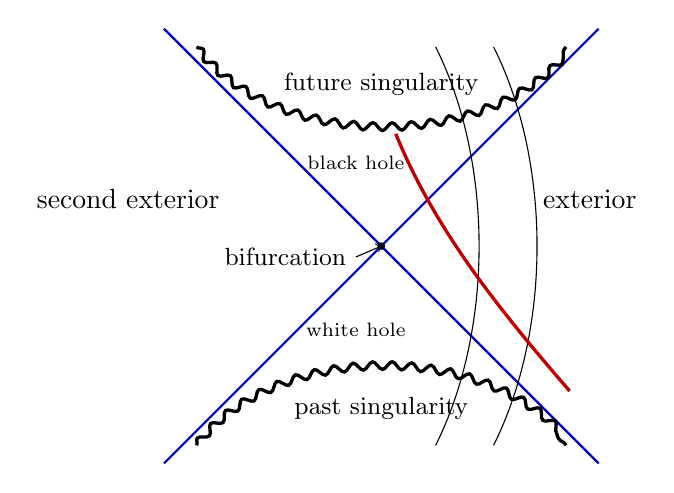
\begin{tikzpicture}[scale=0.92]
\draw[blue!75!black,thick] (-3,-3) -- (3,3);
\draw[blue!75!black,thick] (-3,3) -- (3,-3);
\draw[very thick,decorate,decoration={snake,amplitude=1.4pt,segment length=7pt}]
  (-2.55,2.75) .. controls (-1.45,1.35) and (1.45,1.35) .. (2.55,2.75);
\draw[very thick,decorate,decoration={snake,amplitude=1.4pt,segment length=7pt}]
  (-2.55,-2.75) .. controls (-1.45,-1.35) and (1.45,-1.35) .. (2.55,-2.75);
\draw (0.75,-2.75) .. controls (1.55,-1.15) and (1.55,1.15) .. (0.75,2.75);
\draw (1.55,-2.75) .. controls (2.35,-1.15) and (2.35,1.15) .. (1.55,2.75);
\draw[red!75!black,very thick] (2.6,-2.0) .. controls (1.65,-0.9) and (0.75,0.2) .. (0.2,1.55);
\fill (0,0) circle (1.5pt);
\node[above,font=\small] at (0,1.95) {future singularity};
\node[below,font=\small] at (0,-1.95) {past singularity};
\node[right] at (2.10,0.65) {exterior};
\node[left] at (-2.10,0.65) {second exterior};
\node[font=\scriptsize] at (-0.35,1.15) {black hole};
\node[font=\scriptsize] at (-0.35,-1.15) {white hole};
\node[font=\small,anchor=east] (bifurcation-label) at (-0.35,-0.15) {bifurcation};
\draw[->,thin] (bifurcation-label.east) -- (0,0);
\end{tikzpicture}
\caption{Un diagramme causal non compactifié mis au propre. Les horizons nuls se croisent sur la surface de bifurcation ; les singularités de genre espace se trouvent dans les secteurs futur et passé.}
\end{figure}

\subsection{Possible ne signifie pas typique}

La mécanique microscopique est invariante par renversement du temps à une excellente approximation, pourtant les histoires macroscopiques ont un sens privilégié. Une bombe explose facilement ; les fragments épars se rassemblent presque jamais pour la reconstituer. Une balle dévale facilement un sommet instable ; une balle lancée au hasard ne s’immobilise presque jamais exactement à cet endroit. Un triangle de boules de billard disposées en râtelier se disperse facilement, tandis que les boules éparpillées ne se rangent pas spontanément en triangle. Un glaçon fond dans de l’eau chaude, tandis que l’eau expulse presque jamais un glaçon nouvellement formé.

La distinction tient à l’entropie. Un macroétat de faible entropie occupe une région minuscule de l’espace des phases ; un macroétat de forte entropie correspond à un nombre immense de configurations microscopiques. Les équations autorisent la trajectoire renversée, mais préparer son état microscopique initial exige des corrélations d’une précision extraordinaire.

\begin{classroomqa}
\audiencequestion{Chaque configuration dispersée précise n’est-elle pas aussi improbable que la configuration exacte renversée dans le temps ?\lecturetimestamp{00:56:55}}
\lecturerresponse{Oui, si l’on considère des états microscopiques spécifiés individuellement. L’asymétrie apparaît lorsque l’on compare les macroétats. Une configuration dispersée comprend beaucoup plus d’états microscopiques qu’un triangle assemblé avec précision ; ainsi, presque tous les états microscopiques compatibles avec la première description restent désordonnés à l’échelle macroscopique.}
\end{classroomqa}

Un trou blanc qui émet une Alice parfaitement organisée est la version gravitationnelle d’une telle histoire où l’entropie diminue. Les équations réversibles l’autorisent, mais elle exige un passé extraordinairement particulier. L’horizon porte lui-même de l’entropie et de l’information microscopique cachée ; une fluctuation de la taille d’Alice n’est donc pas logiquement interdite, mais sa probabilité est extrêmement faible.

\begin{classroomqa}
\audiencequestion{Une telle fluctuation serait-elle quantique ou thermique ?\lecturetimestamp{00:59:48}}
\lecturerresponse{Les deux types peuvent contribuer. Dans un système chaud ordinaire, on parle surtout de fluctuation thermique ; pour un trou noir, les effets quantiques et thermiques sont étroitement liés. Dans les deux cas, la forte suppression est essentiellement entropique.}
\end{classroomqa}

\section{Distance propre et compactification de Penrose}

Avant de tracer l’espace-temps global, précisons le vocabulaire radial. Le temps propre est ce que mesure une horloge le long d’une ligne d’univers de genre temps. La distance propre est ce que mesure une chaîne de mètres étalons locaux le long d’une courbe de genre espace choisie. Pour la tranche de Schwarzschild à \(t\) constant,
\begin{equation}
d\rho=\frac{dr}{\sqrt{1-2GM/r}}.
\label{eq:l04-proper-distance}
\end{equation}
Ainsi, \(r\) est une coordonnée aréolaire, et non la distance directe à l’horizon mesurée avec des mètres étalons.

Commençons maintenant par l’espace-temps radial plat. Ne conservons que \(t\) et \(\rho\ge0\). La ligne \(\rho=0\) est l’origine spatiale ; un rayon lumineux radial qui entre dans l’origine poursuit sa trajectoire vers l’extérieur de l’autre côté physique, ce qui apparaît comme une réflexion dans le demi-plan réduit.

Un diagramme de Penrose envoie toutes les valeurs finies et infinies de \(t\) et \(\rho\) dans une région finie, tout en préservant les directions nulles. Il obéit à deux règles :
\begin{enumerate}
\item compactifier tout l’espace-temps en un domaine fini ;
\item conserver les rayons lumineux radiaux à \(45^\circ\).
\end{enumerate}
Les longueurs et les angles ordinaires sont déformés ; les relations causales ne le sont pas.

\begin{figure}[htbp]
\centering
\includegraphics[width=0.70\textwidth]{lecture_04_figure_06.png}
\caption{Grille de compactification achevée pour l’espace-temps de Minkowski radial. Le temps infini se trouve aux extrémités supérieure et inférieure à gauche, et le rayon infini est comprimé jusqu’à la pointe droite.}
\lectureframe{01:14:44.040}
\end{figure}

\begin{figure}[htbp]
\centering
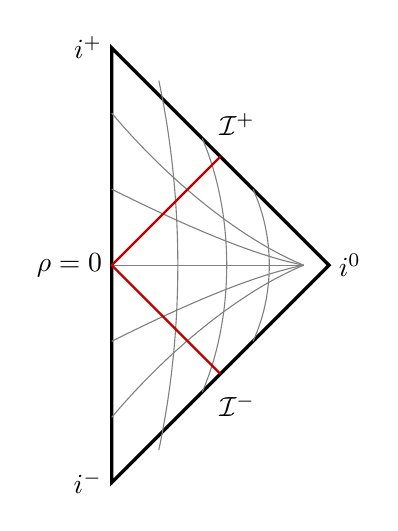
\begin{tikzpicture}[scale=0.92]
\coordinate (im) at (0,-3);
\coordinate (ip) at (0,3);
\coordinate (iz) at (3,0);
\draw[very thick] (im) -- (ip) -- (iz) -- cycle;
\draw[gray] (0,-2.1) .. controls (0.8,-1.15) and (1.8,-0.35) .. (2.65,0);
\draw[gray] (0,-1.05) .. controls (0.9,-0.6) and (1.9,-0.15) .. (2.65,0);
\draw[gray] (0,0) -- (2.65,0);
\draw[gray] (0,1.05) .. controls (0.9,0.6) and (1.9,0.15) .. (2.65,0);
\draw[gray] (0,2.1) .. controls (0.8,1.15) and (1.8,0.35) .. (2.65,0);
\draw[gray] (0.65,-2.55) .. controls (1.0,-0.9) and (1.0,0.9) .. (0.65,2.55);
\draw[gray] (1.25,-1.75) .. controls (1.7,-0.7) and (1.7,0.7) .. (1.25,1.75);
\draw[gray] (1.95,-1.05) .. controls (2.25,-0.4) and (2.25,0.4) .. (1.95,1.05);
\draw[red!75!black,thick] (1.5,-1.5) -- (0,0) -- (1.5,1.5);
\node[left] at (ip) {\(i^+\)};
\node[left] at (im) {\(i^-\)};
\node[right] at (iz) {\(i^0\)};
\node[above right] at (1.35,1.65) {\(\mathcal{I}^+\)};
\node[below right] at (1.35,-1.65) {\(\mathcal{I}^-\)};
\node[left] at (0,0) {\(\rho=0\)};
\end{tikzpicture}
\caption{L’espace-temps de Minkowski radial dans un triangle fini. Le rayon nul rouge arrive depuis \(\mathcal{I}^-\), atteint l’origine et repart par \(\mathcal{I}^+\).}
\label{fig:l04-flat-penrose}
\end{figure}

Les extrémités ont des significations causales distinctes :
\begin{equation}
\begin{aligned}
i^-&:\ \text{past timelike infinity},\\
i^+&:\ \text{future timelike infinity},\\
i^0&:\ \text{spatial infinity},\\
\mathcal{I}^-&:\ \text{past null infinity},\\
\mathcal{I}^+&:\ \text{future null infinity}.
\end{aligned}
\end{equation}
Les symboles \(\mathcal{I}^{-}\) et \(\mathcal{I}^{+}\) se prononcent « scri moins » et « scri plus ».

\begin{classroomqa}
\audiencequestion{Un rayon nul devrait-il passer par les coins de chaque cellule déformée de la grille, et donc être légèrement courbe ?\lecturetimestamp{01:11:08}}
\lecturerresponse{Si l’on traçait exactement la grille complète de coordonnées, ses intersections seraient compatibles avec la courbe nulle. L’idée essentielle est la construction conforme : les directions nulles radiales restent à \(45^\circ\), même si les lignes à \(t\) et à \(\rho\) constants se courbent et se resserrent.}
\end{classroomqa}

\begin{classroomqa}
\audiencequestion{Comment tracer un rayon lumineux s’il ne passe pas par l’origine ?\lecturetimestamp{01:11:45}}
\lecturerresponse{Il atteint une distance minimale non nulle, puis repart vers l’extérieur. Lorsqu’on tient compte du mouvement angulaire, sa trajectoire radiale projetée n’est pas nécessairement une seule droite à \(45^\circ\).}
\end{classroomqa}

\begin{classroomqa}
\audiencequestion{Alors, pourquoi ce rayon lumineux n’est-il pas à \(45^\circ\) ?\lecturetimestamp{01:12:49}}
\lecturerresponse{La règle de \(45^\circ\) a été énoncée pour les rayons lumineux radiaux. Un rayon nul porteur de moment cinétique utilise une partie de son mouvement dans les directions angulaires ; sa projection sur le plan \(t\)-\(\rho\) n’est donc pas radiale.}
\end{classroomqa}

\section{Le diagramme de Schwarzschild éternel}

Le diagramme compactifié comporte quatre régions. Les deux losanges latéraux sont des régions extérieures asymptotiquement plates. Le triangle supérieur est l’intérieur du trou noir et se termine à la singularité future de genre espace. Le triangle inférieur est la région du trou blanc et commence à la singularité passée de genre espace. Ensemble, ces régions forment la géométrie de Schwarzschild maximalement étendue.

\begin{figure}[htbp]
\centering
\includegraphics[width=0.74\textwidth]{lecture_04_figure_07.png}
\caption{Diagramme de Penrose complet de Schwarzschild éternel, avec les singularités, les horizons, les trajectoires nulles et une frontière asymptotique indiqués au tableau.}
\lectureframe{01:21:30.000}
\end{figure}

\begin{figure}[htbp]
\centering
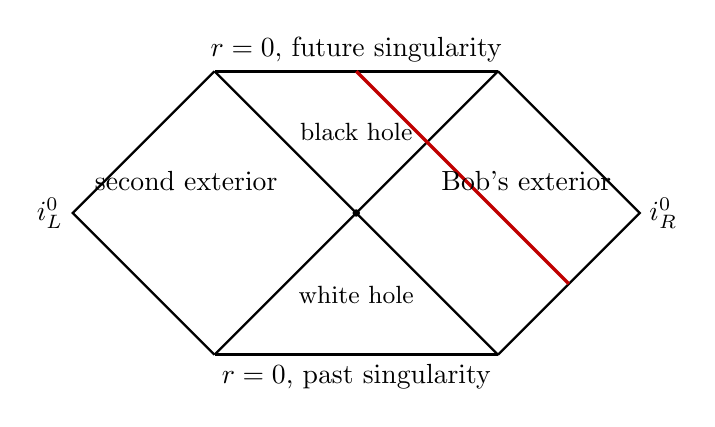
\begin{tikzpicture}[scale=0.90]
\coordinate (C) at (0,0);
\coordinate (TL) at (-2,2);
\coordinate (TR) at (2,2);
\coordinate (BL) at (-2,-2);
\coordinate (BR) at (2,-2);
\coordinate (L) at (-4.0,0);
\coordinate (R) at (4.0,0);
\draw[very thick] (TL) -- (TR);
\draw[very thick] (BL) -- (BR);
\draw[thick] (C) -- (TL) (C) -- (TR) (C) -- (BL) (C) -- (BR);
\draw[thick] (TL) -- (L) -- (BL);
\draw[thick] (TR) -- (R) -- (BR);
\draw[red!75!black,very thick] (3,-1) -- (1,1) -- (0,2);
\node[above] at (0,2) {\(r=0\), future singularity};
\node[below] at (0,-2) {\(r=0\), past singularity};
\node[font=\small] at (0,1.15) {black hole};
\node[font=\small] at (0,-1.15) {white hole};
\node at (2.4,0.45) {Bob's exterior};
\node at (-2.4,0.45) {second exterior};
\node[right] at (R) {\(i^0_R\)};
\node[left] at (L) {\(i^0_L\)};
\fill (C) circle (1.5pt);
\end{tikzpicture}
\caption{Les quatre régions de Schwarzschild éternel. Un rayon lumineux radial entrant traverse l’horizon futur et se termine en \(r=0\).}
\label{fig:l04-eternal}
\end{figure}

Un rayon lumineux radial entrant depuis \(\mathcal{I}^-\) traverse l’horizon futur et se termine sur la singularité. Toute courbe causale du triangle supérieur connaît le même sort. On décrit souvent le second extérieur comme l’autre bouche d’un pont d’Einstein--Rosen, mais celui-ci n’est pas traversable : tout trajet causal tenté d’un extérieur à l’autre pénètre dans la région du trou noir et atteint la singularité.

\begin{classroomqa}
\audiencequestion{Les deux univers extérieurs sont-ils reliés par un trou de ver, et peut-on y transmettre un signal ?\lecturetimestamp{01:22:21}}
\lecturerresponse{La géométrie éternelle contient un pont d’Einstein--Rosen sur certaines tranches spatiales, mais aucun signal causal ne passe d’un extérieur à l’autre. Le pont se referme trop vite ; même la lumière qui franchit un horizon se termine à la singularité future.}
\end{classroomqa}

Ce diagramme décrit un trou qui existe depuis toujours. Les trous astrophysiques réels se forment à partir de matière en effondrement. Leur diagramme causal ne comporte ni singularité passée de trou blanc ni second extérieur asymptotique. Pour construire cette géométrie, il nous faut comprendre les coquilles sphériques.

\section{Former un trou noir par effondrement}

Imaginons une coquille sphérique diffuse de particules entrantes. Il peut s’agir de photons : l’énergie gravite, si bien qu’une impulsion de rayonnement suffisamment concentrée peut former un trou noir. Avant l’effondrement, la région centrale ressemble à un espace-temps plat vide ; une fois l’énergie suffisamment comprimée, l’extérieur ressemble à l’espace-temps de Schwarzschild. Il s’agit de raccorder ces régions de part et d’autre de la coquille en mouvement.

\subsection{Théorème des coquilles de Newton}

Pour une coquille newtonienne sphérique de masse totale \(M\), la loi de Gauss pour la gravitation s’écrit
\begin{equation}
\oint \mathbf{g}\cdot d\mathbf{A}=-4\pi G M_{\mathrm{enc}}.
\label{eq:l04-gauss-gravity}
\end{equation}
La symétrie sphérique implique que \(\mathbf{g}=g(r)\hat{\mathbf r}\), donc
\begin{equation}
g(r)=
\begin{cases}
0, & r<R_{\mathrm{shell}},\\[4pt]
-\dfrac{GM}{r^2}, & r>R_{\mathrm{shell}}.
\end{cases}
\label{eq:l04-shell-field}
\end{equation}
À l’intérieur, aucune masse n’est enfermée et le champ gravitationnel s’annule. À l’extérieur, la coquille agit exactement comme une masse ponctuelle \(M\) placée au centre. Le potentiel est constant à l’intérieur plutôt que nul, mais il ne subsiste aucune force newtonienne locale.\editorialnote{L’argument par les lignes de champ présenté en cours est formulé précisément par la loi de Gauss. La distinction entre champ nul et potentiel constant importe lorsqu’on compare les normalisations des horloges en relativité.}

Cette conclusion reste valable tant qu’une coquille parfaitement sphérique se contracte, pourvu que sa masse totale soit conservée. Seule la position de la frontière entre les solutions intérieure et extérieure change.

\subsection{Théorème de Birkhoff}

L’équivalent relativiste est le théorème de Birkhoff : toute région de vide sphériquement symétrique est localement une portion de la famille de Schwarzschild. Pour une coquille sans masse en son centre,
\begin{align}
ds^2_{\mathrm{inside}}&=-dT^2+dR^2+R^2d\Omega_2^2,\\
ds^2_{\mathrm{outside}}&=
-\left(1-\frac{2GM}{r}\right)dt^2
\nonumber\\
&\quad+\frac{dr^2}{1-2GM/r}
+r^2d\Omega_2^2.
\label{eq:l04-birkhoff-pieces}
\end{align}

\begin{figure}[htbp]
\centering
\includegraphics[width=0.74\textwidth]{lecture_04_figure_08.png}
\caption{Schéma du raccordement à la coquille : espace-temps plat à l’intérieur du cercle et solution de Schwarzschild à l’extérieur.}
\lectureframe{01:34:15.000}
\end{figure}

\begin{classroomqa}
\audiencequestion{Quelle métrique trouve-t-on à l’extérieur d’une coquille sphérique en relativité générale ?\lecturetimestamp{01:33:17}}
\lecturerresponse{La métrique de Schwarzschild, dont le paramètre de masse est égal à la masse totale conservée de la coquille. La région centrale vide est localement l’espace-temps de Minkowski.}
\end{classroomqa}

\begin{classroomqa}
\audiencequestion{Si la coquille se contracte, pourquoi le paramètre de masse ne change-t-il pas ?\lecturetimestamp{01:34:33}}
\lecturerresponse{Parce que l’énergie totale est conservée. Le rayon de la coquille ainsi que ses contributions cinétiques ou de liaison peuvent changer, mais la masse extérieure conservée est fixe pour un système sphérique isolé. La coquille en mouvement change l’emplacement du raccordement entre les régions plate et de Schwarzschild.}
\end{classroomqa}

Un intérieur plat ne signifie pas que l’horloge située à l’intérieur ait nécessairement la même normalisation que celle située à l’infini. Le raccordement à travers la coquille peut multiplier la coordonnée temporelle intérieure par une constante, et une coquille en mouvement impose les conditions de raccordement correspondantes.\editorialnote{Le théorème de Birkhoff détermine localement chaque région vide. La relation globale entre leurs coordonnées est fixée par le raccordement de la métrique induite et de la courbure extrinsèque de part et d’autre de la coquille. Ces détails sont reportés, tout comme la construction de l’effondrement est reportée à la prochaine leçon.}

Nous disposons maintenant des deux éléments nécessaires à la formation : l’espace-temps de Minkowski à l’intérieur de la coquille en contraction et l’espace-temps de Schwarzschild à l’extérieur. À mesure que la coquille se déplace vers l’intérieur, leur interface décrit un tube d’univers. Le passage de ce tube d’univers à travers le rayon de Schwarzschild remplacera la moitié passée non physique de la figure~\ref{fig:l04-eternal}par une région régulière antérieure à l’effondrement et révélera où commence l’horizon des événements d’un véritable trou noir.
